\documentclass{article}

% various packages and settings {{{

% math packages
\usepackage{amsmath, amsfonts, mathtools}

% other important packages (should stay on top)
\usepackage{graphicx, multicol, xcolor}

% change to German
\usepackage[german]{babel}

% utf8 characters
\usepackage[utf8]{inputenc}

% font
\usepackage[scaled]{helvet}
\renewcommand{\familydefault}{\sfdefault}
\usepackage[]{fontspec}

% fontsize
\usepackage[12pt]{extsizes}

% no paragraph indents
\setlength{\parindent}{0pt}

% better hyphenation
\usepackage[final]{microtype}
\usepackage{csquotes}

% import line spacing
\usepackage{setspace}

% page format
\usepackage{geometry}
\geometry{
    a4paper,
    left=25mm,
    right=25mm,
    top=25mm,
    bottom=25mm
}
    
% page header
\usepackage{fancyhdr}
\pagestyle{fancy}
\fancyhf{}
\lhead{\textbf{\today}}
\rhead{\textbf{Induktion}}

% }}}

\begin{document}

% set line spacing
\setstretch{1.5}

\section*{Änderung des Magnetfelds}

\subsection*{Versuch}

\begin{multicols}{2}
    Beim Versuch wird eine Spule mit angeschlossenem Voltmeter in den Wirkbereich
    einer 2. magnetfelderzeugenden Spule gebracht. Diese ist an eine regelbare
    Gleichstromquelle mit Sägezahngenerator angeschlossen, sodass sich die
    Spannung gleichmäßig ändert.

    \columnbreak
    \begin{center}
        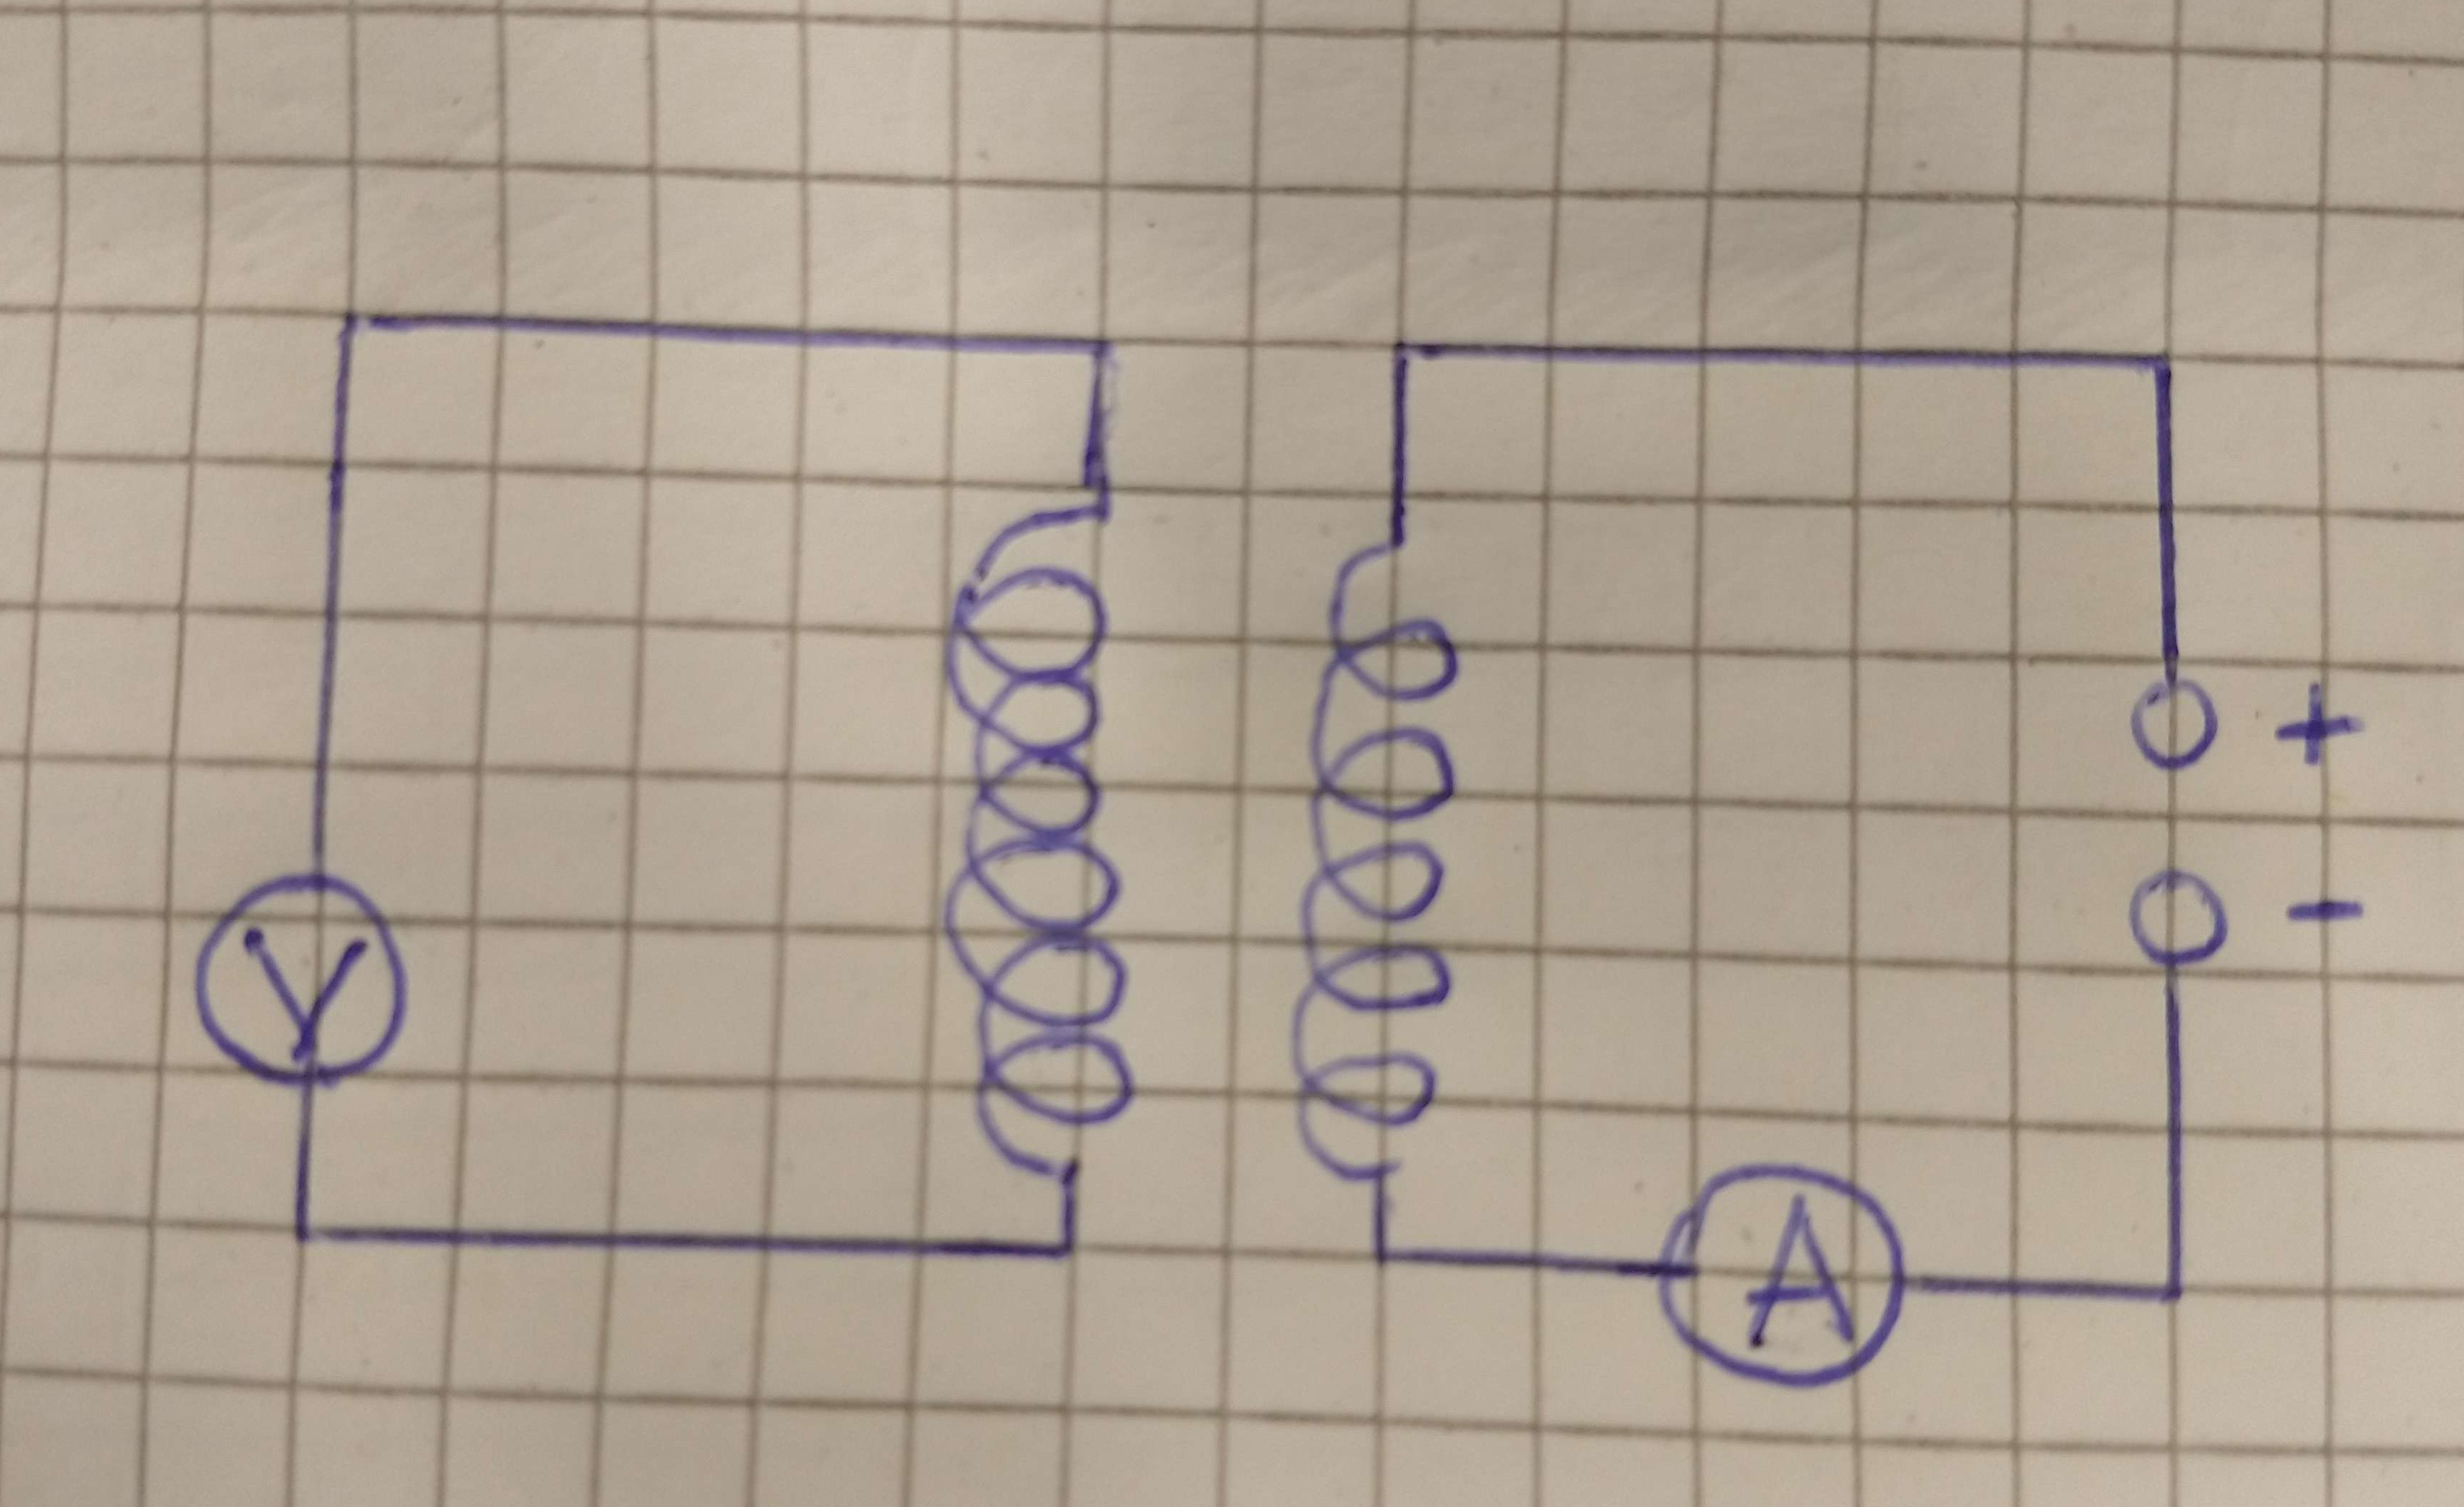
\includegraphics[width=7cm]{./images/induktion_versuch_spulen_haendisch.jpg}
    \end{center}

\end{multicols}

\subsection*{Durchführung und Ergebnisse}

\begin{multicols}{2}

    \textbf{Durchführung:}

    Man stellt die Stromquelle auf eine konstante Spannungsänderung ein.
    Anschließend startet man den Steigerungsprozess und kann eine Induktionsspannung
    am Voltmeter ablesen. Außerdem lässt sich die Stromstärke der Magnetfelderzeugenden
    Spule ablesen. So erhält man Daten, die man in Zusammenhang bringen kann.
    \columnbreak

    \textbf{Ergebnisse:} \\
    Es ergibt sich, dass die Induktionsspannung bei schnellerem Anstieg der Spannung,
    also einer größeren Änderung des Magnetfelds, größer ist.
    Es besteht ein proportionaler Zusammenhang.
    \newline

    \Large
    \hspace{1cm}$U_{i} \propto \Delta B$

\end{multicols}

\subsection*{Formel zur Berechnung}
Unter Einbezug von Wicklungsanzahl der Spule und Fläche, als Querschnitt des Leiters,
ergibt sich folgendes.
\newline

\normalsize
Berechnung der Induktionsspannung, wenn sich das Magnetfeld um den Leiter ändert:
\newline

\Large
$U_{i} = n \cdot A \cdot \frac{\Delta B}{\Delta t}$

\newpage

\section*{Bewegung des Leiters}

\subsection*{Herleitung der Formel aus $F_{el}$ und $F_{L}$}

Bekannte Formeln:
\newline

\Large
$F_{el} = e \cdot E$

$F_{L} = e \cdot v \cdot B$

$E = \frac{U}{l}$
\newline

\normalsize
Zur Herleitung wird der Ansatz der Kräftegleichheit genutzt.
Bewegt sich ein Leiter in einem Magnetfeld, so wirkt die Lorenzkraft, welche
gleich ist zur elektrischen Kraft, der Spannung, die so im Leiter herrscht.
\newline

\Large
$F_{el} = F_{L}$

$e \cdot E = e \cdot v \cdot B$ \hspace{0.25cm}$| :e$

$E = v \cdot B$

$\frac{U}{l} = v \cdot B$ \hspace{0.25cm}$| \cdot l $

$U = v \cdot B \cdot l$
\newline

\normalsize
Die Anzahl der Windungen der Spule sorgt für die Multiplikation des Faktors
$n$. $U$ ist gleich der induzierten Spannung $U_{i}$.
Dabei ist $l$ die effektive, und nicht die reale, Leiterlänge.
\newline

\normalsize
Berechnung der Induktionsspannung, wenn sich der Leiter im Magnetfeld bewegt:
\newline

\Large
$U_{i} = n \cdot v \cdot B \cdot l$

\newpage

\section*{Zusammenführung der Einzelformeln}

\subsection*{Grundlagen der Formeln}

\normalsize
Berechnung der Induktionsspannung, wenn sich der Leiter im Magnetfeld bewegt:
\newline

\Large
$U_{i_1} = n \cdot v \cdot l \cdot B$
\newline

\normalsize
Berechnung der Induktionsspannung, wenn sich das Magnetfeld um den Leiter ändert:
\newline

\Large
$U_{i_2} = n \cdot A \cdot \frac{\Delta B}{\Delta t}$
\newline

\normalsize
Ansätze der Umformung:
\newline

\Large
$v = \frac{\Delta s}{\Delta t}$
\newline

\normalsize
Zuerst wird die Gleichung $U_{i_1}$ umgeformt.
\newline

\Large
$U_{i_1} = n \cdot v \cdot l \cdot B$

$U_{i_1} = n \cdot \frac{\Delta s}{\Delta t} \cdot l \cdot B$
\newline

\normalsize
Aus den 2 Strecken ergibt sich eine Fläche. Diese Fläche ist der Bereich an
Feldlinien, die der Leiter in der Bewegung durchläuft.
\newline

\Large
$U_{i_1} = n \cdot \frac{\Delta A}{\Delta t} \cdot B$

\newpage

\subsection*{Zusammenführen}

\normalsize
Die Gesamtinduktionsspannung ergibt sich sowohl aus der Bewegung des Leiters
als auch der Änderung des Magnetfelds.
\newline

\Large
$U_{i} = U_{i_1} + U_{i_2}$

\vspace{0.3cm}
$U_{i} = n \cdot \frac{\Delta A}{\Delta t} \cdot B + n \cdot A \cdot \frac{\Delta B}{\Delta t}$ \hspace{0.25cm}$|$ \normalsize Ausklammern

\vspace{0.3cm}
\Large
$U_{i} = n \cdot (\frac{\Delta A}{\Delta t} \cdot B + A \cdot \frac{\Delta B}{\Delta t})$  \hspace{0.25cm}$|$ \normalsize physikalische Notierung

\vspace{0.3cm}
\Large
$U_{i} = n \cdot (\dot{A} \cdot B + A \cdot \dot{B})$ \hspace{0.25cm}$|$ \normalsize Umformung mit Produktregel

\vspace{0.3cm}
\Large
$U_{i} = n \cdot \dot{(A \cdot B)}$  \hspace{0.25cm}$|$ \normalsize Phi als physikalische Symbol

\vspace{0.3cm}
\Large
$U_{i} = n \cdot \dot{\Phi}$
\newline

\normalsize
Die Induktionsspannung lässt sich aus der Windungsanzahl $n$ und der Änderung des
magnetischen Kraftfluss $\dot{\Phi}$ berechnen.

\newpage

\section*{Selbstinduktion}

\setlength{\columnsep}{2.5cm}

\subsection*{Induktionsregeln}

\normalsize
\begin{multicols}{2}
    Die Selbstinduktion bezeichnet den Vorgang, wenn eine magnetfelderzeugende Spule
    in sich selbst eine Induktionsspannung erzeugt. Dabei ist die Richtung dieser
    Induktionsspannung durch die lenzsche Regel bestimmt.

    \columnbreak


    \setlength\fboxsep{0.4cm}

    \noindent\fcolorbox{red}{white}{%
        \parbox{7cm}{
            \textbf{Lenzsche Regel}:
            Bei Änderung des magnetischen Flusses in einer Spule wird eine Spannung induziert,
            welche der Änderung des magnetischen Flusses entgegenwirkt.
        }
    }

\end{multicols}

\subsection*{Lampenversuch}

\begin{multicols}{2}
    Die Lampe im Stromkreis mit der Spule leuchtet später.
    Dies liegt daran, dass die Selbstinduktionsspannung der Spannung
    des Stromkreis entgegenwirkt und so die Gesamtspannung bei der Lampe
    geringer ist.


    \columnbreak

    \begin{center}
        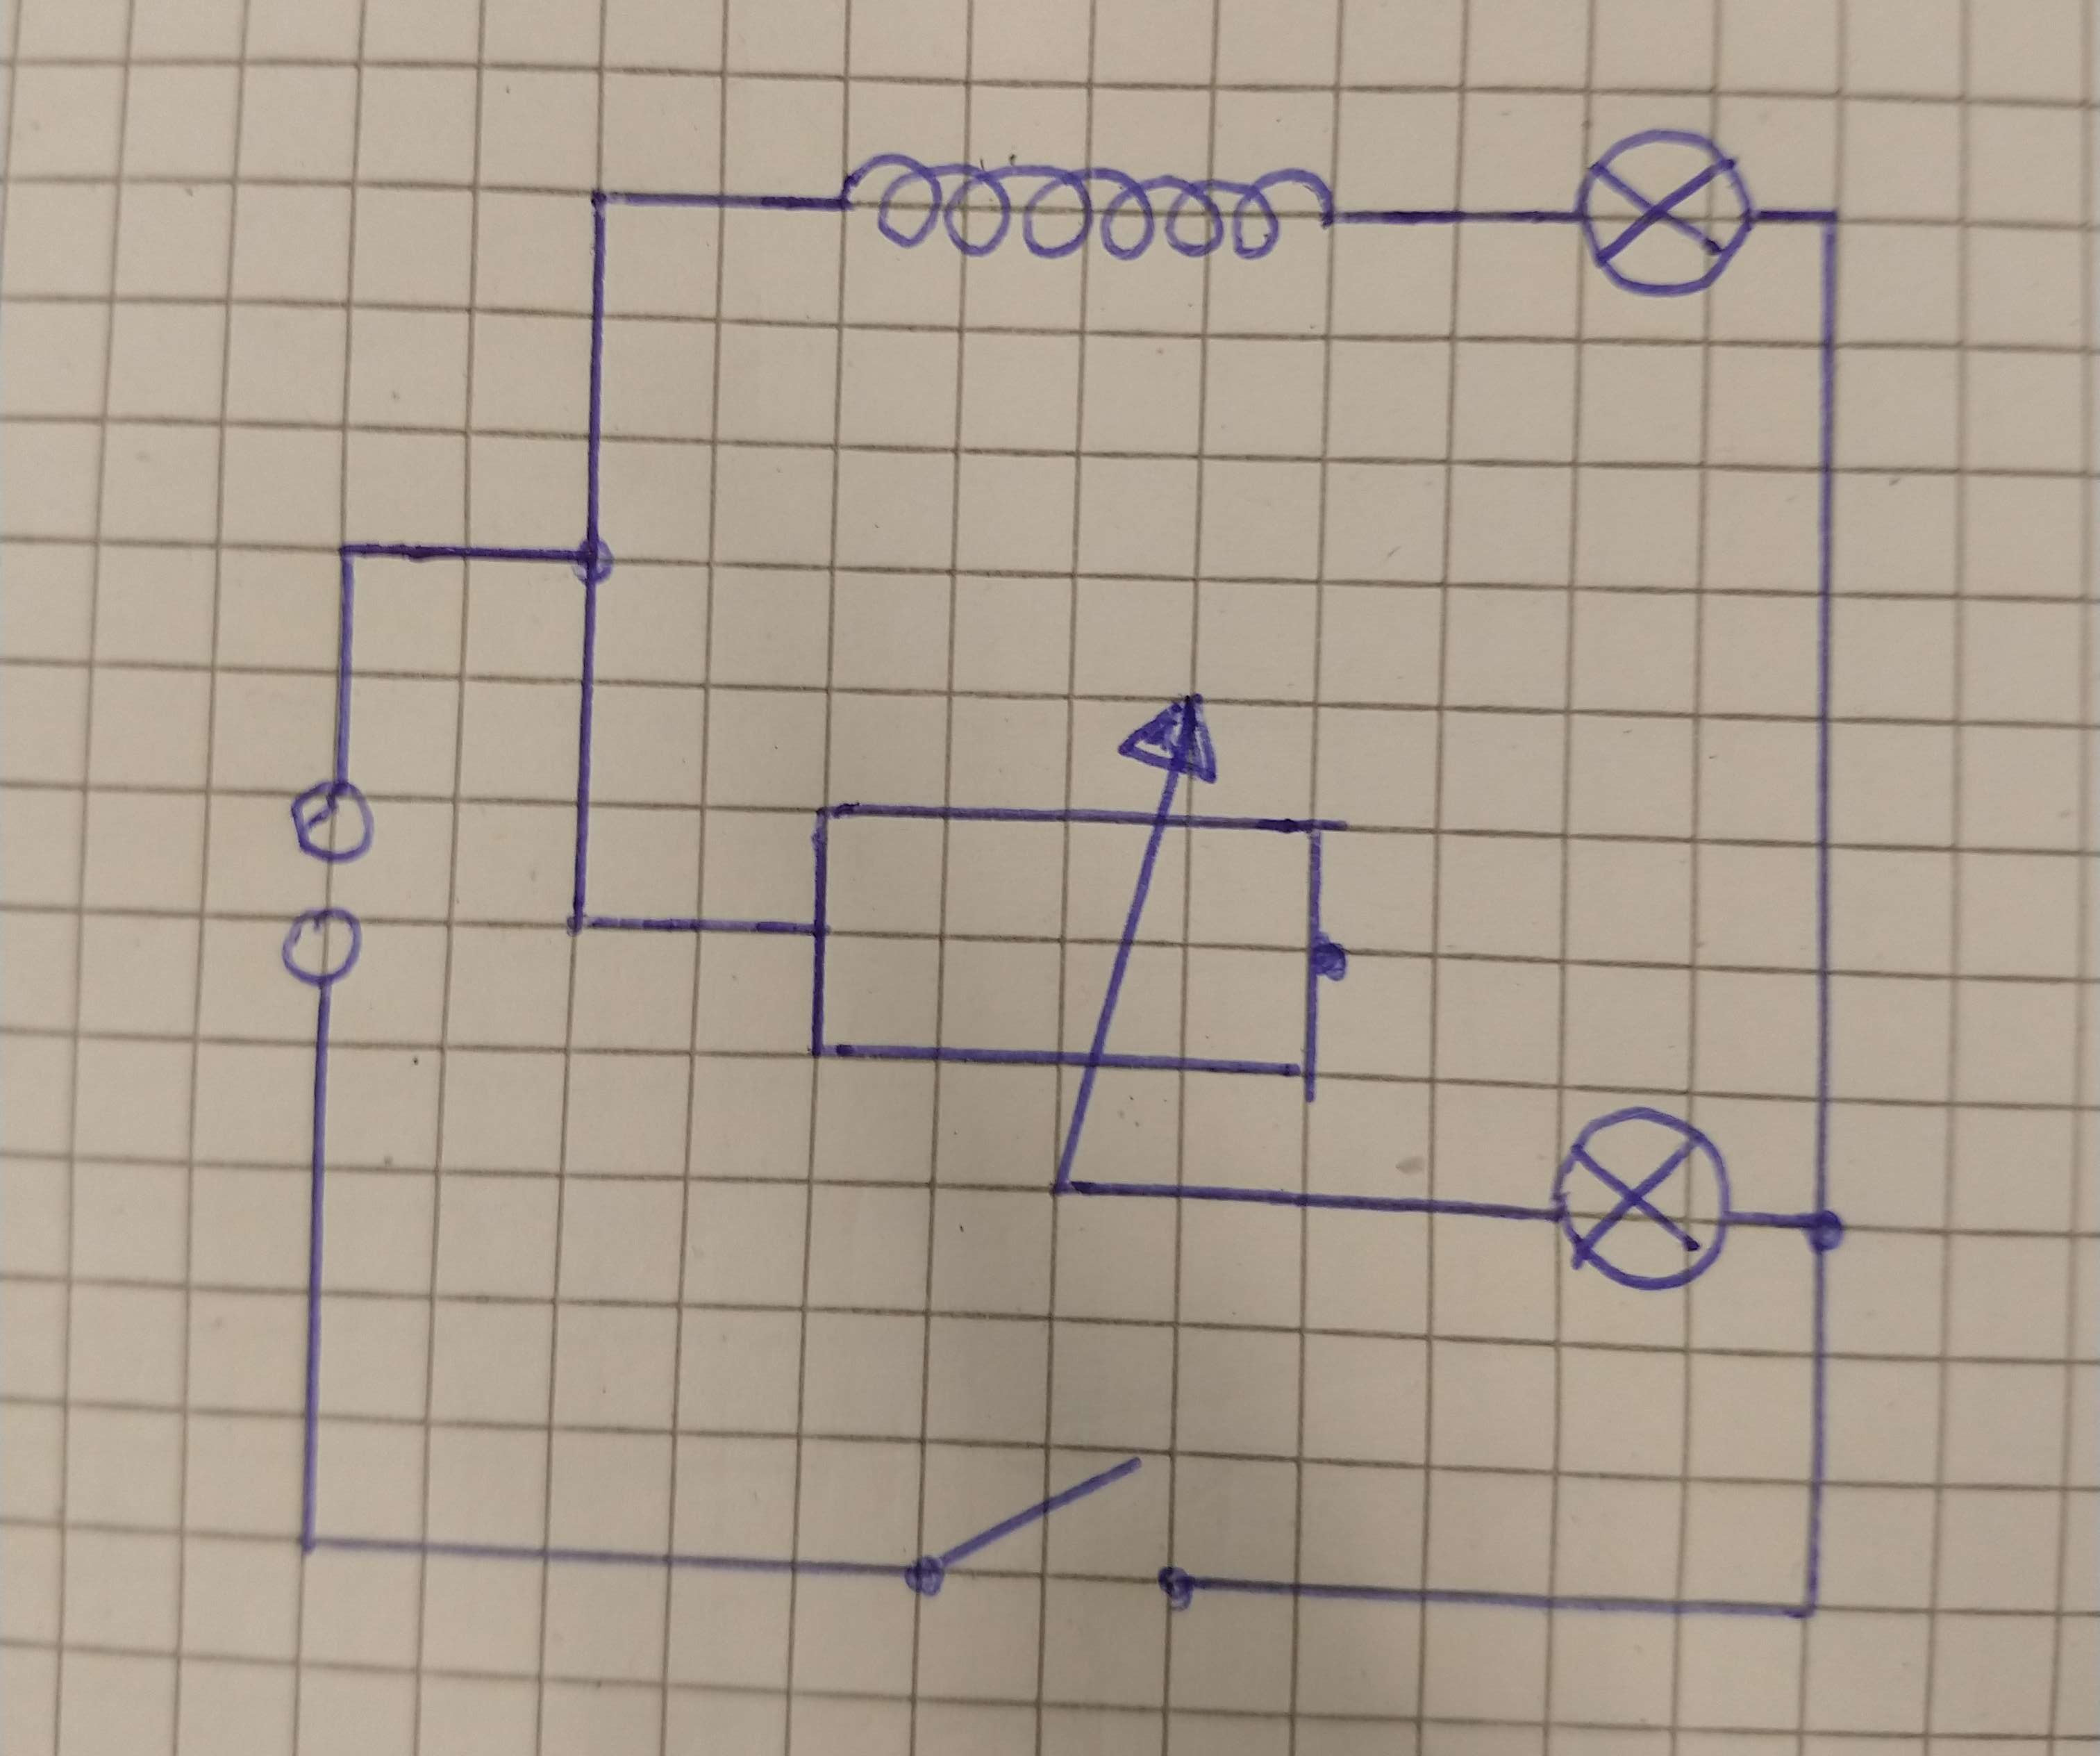
\includegraphics[width=7cm]{./images/induktion_versuch_widerstand_laenge_haendisch.jpg}
    \end{center}

\end{multicols}

\subsection*{Induktivität von Spulen}

Die Induktivität einer Spule beschreibt die Induktionsfähigkeit und
beschreibt unter anderem die Stärke der Selbstinduktion.
\newline

\Large
$L = \mu_0 \cdot \mu_r \cdot \frac{N^2 \cdot A}{l}$
\newline

\normalsize
Die Einheit der Induktivität ist Henry.
\newline

\Large
$[L] = 1H = 1VsA^{-1}$

\end{document}
